\chapter{Evaluation}
\label{cha:evaluation}


In the following chapter we use three different methods to evaluate our results. First we compute the nearest neighbors of different word senses. Then we use the t-SNE approach to project the embedding vectors to two dimensions and visualize semantic similarity. Finally we perform the  WordSim-353 task proposed by \cite{FinkelsteinGabrilovichEtAl2001} and the Contextual Word Similarity (SCWS) task from \cite{HuangSocherEtAl2012}.

The WordSim-353 dataset is made up by 353 pairs of words followed by similarity scores from 10 different people and an average similarity score. The SCWS Dataset has 2003 words pairs with their context respectively, which also contains 10 scores from 10 different people and an average similarity score. The task is to reproduce these similarity scores. 

For the WordSim-353 dataset, we use the $avgSim$ function to calculate the similarity score of two words $w,\tilde{w}\in D$ from our model as following
\begin{equation}
avgSim(w,\tilde{w})
=\frac{1}{N_w}\frac{1}{N_{\tilde{w}}}\sum_{i=1}^{N_w}\sum_{j=1}^{N_{\tilde{w}}}\cos(V_{w,i},V_{\tilde{w},j})
\end{equation}

where $\cos(x, y)$ denotes the cosine similarity score of vectors $x$ and $y$, $N_w$ means the number of senses for word $w$, and $V_{w,i}$ represents the $i$-th sense input embedding vector of word $w$. 

Cosine similarity is a measure of similarity between two vectors of an inner product space that measures the cosine of the angle between them \footnote{https://en.wikipedia.org/wiki/Cosine$\_$similarity}. Specifically, given two vectors $a$ and $b$ with the save dimension $d$, the cosine similarity of them is
$$cos(a,b)=\frac{\sum_{i=1}^d a_i b_i}{\sqrt{\sum_{i=1}^d {a_i}^2}\sqrt{\sum_{i=1}^d {b_i}^2}}$$

The SCWS task is similar as the \textbf{Assign} operation. We use a center word to predict the context words. But here we do not do the real assignment for whole sentence which needs several times to assign until it is stable. Actually, our sense output embedding has only one sense. So we just use the normal skip-gram model's prediction function to select the best center word's sense.

In order to evaluate our model, after getting the similarity score for each pair of words, we use Spearman’s rank correlations to calculate the correlation between the similarity scores from our model and the given similarity scores from SCWS and word353 datasets. The higher correlation represents the better result. The definition details can be referred in Wikipedia\footnote{https://en.wikipedia.org/wiki/Spearman$\%$27s$\_$rank$\_$correlation$\_$coefficient}. 



\section{Results for different Hyper-Parameters}

\begin{table}[tb]
	\caption{Definition of Hyper-Parameters of the Experiments } \label{tab:notationhyper}
	\begin{center}
		\begin{tabular}{|l|l|}
			\hline
			\multicolumn{2}{|l|}{\bf Fixed Parameters}  \\ \hline
			$numRDD$=20 & The number of RDD to split training data set.\\ \hline
			\gls{c}=5& The size of context  \\ \hline
			\gls{K}=10& The number of negative samples\\ \hline
			\multicolumn{2}{|l|}{\bf Variable Parameters}  \\ \hline
			$id$ & The id number of the experiment. \\ \hline
			$c1$ &  Minimal count for the inclusion of a word the in vocabulary $D$\\ \hline
			\gls{d} & Vector size for each embedding vector  \\ \hline
			\multirow{2}{*}{$c2$} 
			&  Count thresholds for words with two senses\\
			&  i.e. the count of $w$ is more than $c2$, $w$ has at least two senses\\ 
			\hline
			\multirow{2}{*}{$c3$} 
			&  Count thresholds for words with three senses\\
			&  i.e. the count of $w$ is more than $c3$, $w$ has at least three senses\\ \hline
			$lr$ &  The learning rate at the beginning of the experiment.\\ \hline
			$gm$ &  The reduction factor of the learning rate for each iteration\\ \hline
			$S1$ & true if sense has only one output embedding vector\\ 
			\hline
		\end{tabular}
	\end{center}
\end{table}


\begin{table}[tb]
	\caption{Definition of Evaluation Scores } \label{tab:notationevalution}
	\begin{center}
		\begin{tabular}{|l|l|}
			\hline 
			$t1$ & The average time of learning parameters in one iteration  \\ \hline
			$t2$ & The average time of collecting parameters using $treeAggregate$ in one iteration \\ \hline
			
			$t3$ &The average time of all operations in one iteration \\ \hline
			
			$t4$ & Total training time \\ \hline
			$iter$ & The number of total training iterations \\ \hline
			$vLoss$ & The best loss of the validation set \\ \hline
			$SCWS$ & The Spearman’s rank correlations on the SCWS dataset. 
			\\ \hline
			$word353$ & The Spearman’s rank correlations on the word353 dataset \\ \hline
			
		\end{tabular}
	\end{center}
\end{table}

Different hyper-parameters can generate different loss values on the validation set and require different computation time and memory. We tried many different parameters and found that the number of negative samples, the window size are not the typical factors to affect the final results. From the experiments we choose $c=5$, the size of the $Context(w_t)$, i.e. the number of words before and after $w_t$.
The number of negative samples $K$ randomly generated for a word was set to $10$.

And we also found that it is better to choose $numRDDs = 20$, which can balance the time of learning parameters and the time of collecting parameters. So in the following analysis, we do not change these three hyper-parameters only focus on other hyper-parameters, and Table \ref{tab:notationhyper} shows the hyper-parameters we need. And we mainly use the time, the loss and the score of similarity task shown as Table \ref{tab:notationevalution} to compare these hyper-parameters. 

Note that we need two steps to train sense embedding vectors. In Step~1 the number of all word senses is set to one and the word embedding vectors are trained as in the usual word2vec approach. In Step~2 the program will use the result from Step~1 to do initialization of senses vectors (adding a tiny noise) and then train the sense embedding vectors. Finally, we decide to list only 11 experiments on Step 2 shown as Table \ref{tab:experiment11}, which are based on 8 experiments on Step 1 shown as Table \ref{tab:experiment8}. 




\begin{table}[tb] 
\caption{8 Different Experiments in Step 1} \label{tab:experiment8}
\begin{center}
\begin{tabular}{|l|l|l|l|l|}
\hline
id&c1&vec&lr&gm \\ \hline
(1) 	&  200 		& 300  	& 0.1		& 0.9	\\ \hline
(2) 	&  200 		& 250  	& 0.1		& 0.9	\\ \hline
(3) 	&  200 		& 200  	& 0.1		& 0.9	\\ \hline
(4) 	&  200 		& 150  	& 0.1		& 0.9	\\ \hline
(5) 	&  200 		& 100  	& 0.1		& 0.9	\\ \hline
(6) 	&  200 		& 50 	& 0.1		& 0.9	\\ \hline
(7)	&  20		& 50	& 0.1		& 0.9	\\ \hline
(8)	&  20		& 50	& 0.01		& 0.95	\\ \hline
\end{tabular}
\end{center}
\end{table}


\begin{table}[tb]

\caption{11 Different Experiments in Step 2} \label{tab:experiment11}
\begin{center}
\begin{tabular}{|l|l|l|l|l|l|l|l|}
\hline
id&c1&vec&cm&lr&gm&syn1&init \\ \hline
1 	&  200 		& 300 	& 2000$\_$10000 	& 0.1		& 0.9	& true & (1)\\ \hline
2	&  200		& 250   & 2000$\_$10000 	& 0.1		& 0.9	& true & (2)\\ \hline
3	&  200		& 200   & 2000$\_$10000 	& 0.1		& 0.9	& true & (3)\\ \hline
4	&  200		& 150   & 2000$\_$10000 	& 0.1		& 0.9	& true & (4)\\ \hline
5 	&  200 		& 100 	& 2000$\_$10000 	& 0.1		& 0.9	& true & (5) \\ \hline
6 	&  200 		& 50 	& 2000$\_$10000 	& 0.1		& 0.9	& true & (6)\\ \hline
7	&  20		& 50	& 2000$\_$10000	& 0.1		& 0.9	& true & (7)\\ \hline
8	&  20		& 50	& 2000$\_$10000	& 0.01		& 0.95	& true & (8)\\ \hline
9 	&  20		& 50 	& 2000$\_$100000 	& 0.1		& 0.9	& true & (7)\\ \hline
10 	&  20		& 50 	& 7000$\_$10000 	& 0.1		& 0.9	& true & (7)\\ \hline
11 	&  20		& 50 	& 2000$\_$10000 	& 0.1		& 0.9	& false& (7)\\ \hline
\end{tabular}

\end{center}
\end{table}

In the following, we build 5 comparison groups based these 11 experiments to check how these hyper-parameters affect the final validation loss, the convergence speed, training time and similarity task scores. 

\paragraph{Different sizes of embedding vectors} \ \\
From the comparison in Table \ref{tab:group1}, it is clear that the bigger embedding vector size can get smaller $vLoss$, bigger $SCWC$ and smaller $word353$. 

\begin{table}[tb]
\caption{Different Vector Size Comparison} \label{tab:group1} 
\begin{center}
\begin{tabular}{|l|l|l|l|l|l|l|l|l|l|}
\hline
$id$ & $K$  & $t1$ & $t2$ & $iter$ & $t3$ & $t4$ &   $vLoss$  & 	$SCWS$ & 	$word353$	   \\ 
\hline
1 	& 300 	& 947.8	& 842	& 35	& 2272.9 &	79550  & 0.2437 &0.5048 & 0.5233  \\ 
\hline
2 	& 250 	& 764.7& 533	& 35	& 1755.7 &	61450  & 0.2437 &0.5083 & 0.5271 \\ 
\hline
3 	& 200 	& 632.5& 322	& 40	& 1389.9 &  55593  & 0.2436 &0.5103 & 0.5371 \\ 
\hline
4 	& 150 	& 502.7& 210	& 35	& 1069.9 &	37448  & 0.2440 &0.5048 & 0.5233 \\ 
\hline
5 	& 100 	& 494.7	& 70.1	& 35	& 827.30 &	28956  & 0.2446 &0.4994 & 0.5355  \\ 
\hline
6 	& 50 	& 342.9& 34.6	& 35	& 683.29 &	23915  & 0.2458 &0.4666 & 0.5449  \\ 
\hline
\end{tabular}
\end{center}
\end{table}


\begin{figure}[tb]
  \centering
	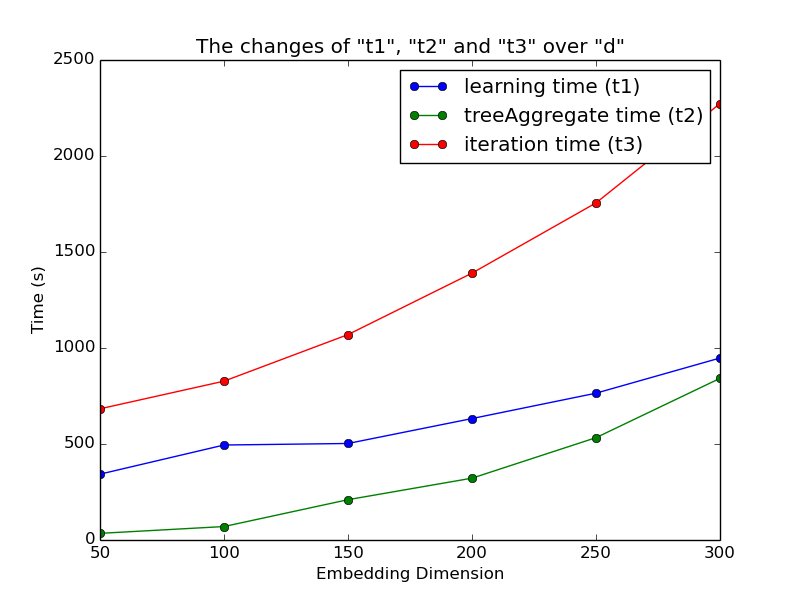
\includegraphics[width=0.8\textwidth]{vectime} 
	\caption{Shows the effect of varying embedding dimensionality of our Model on the Time}
	\label{fig:vec_time}
\end{figure}

\begin{figure}[!ht]
  \centering
	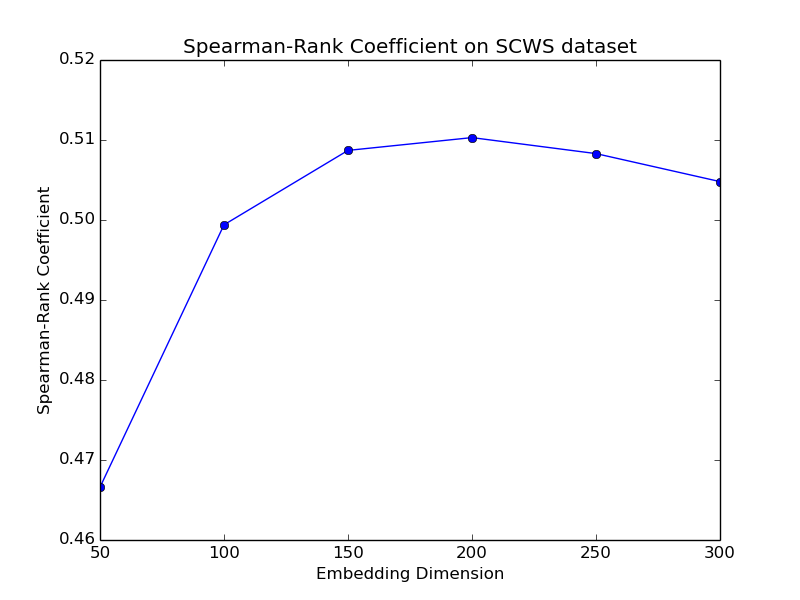
\includegraphics[width=0.7\textwidth]{vecSCWS} 
	\caption{Shows the effect of varying embedding dimensionality of our Model on the SCWS task}
	\label{fig:vecSCWS}
\end{figure}


\begin{figure}[tb]
  \centering
	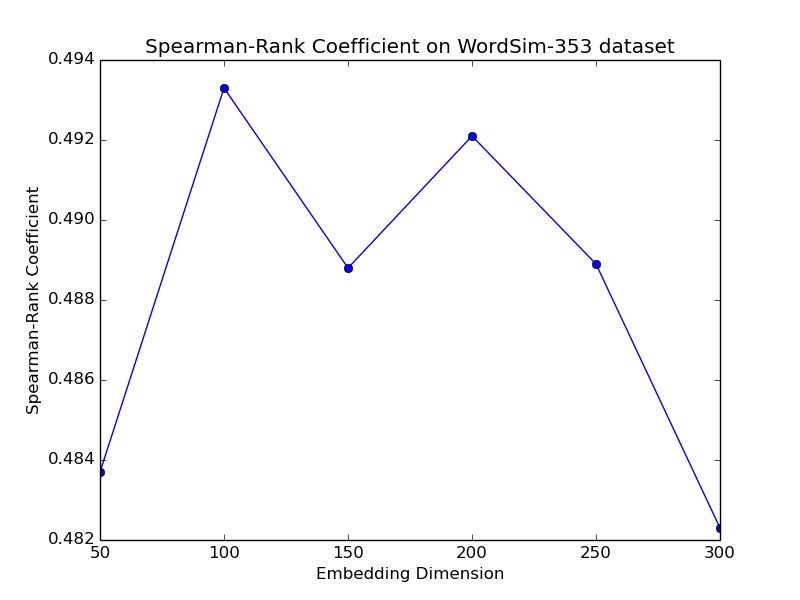
\includegraphics[width=0.7\textwidth]{vecword353} 
	\caption{Shows the effect of varying embedding dimensionality of our Model on the word353 task}
	\label{fig:vecword353}
\end{figure}




\paragraph{Different Min Count} \ \\
We can find from Table \ref{tab:group2} that the size of dictionary is not the important factor influencing loss or performance of similarity tasks. A higher $minCount$ remove some words from the vocabulary which are not frequent. As we know , each word's embedding vector is trained based on the surrounding words. Since those words are infrequent, each of them enters the training of frequent words only in a small amount. So they won't affect the final embedding vectors of frequent words.

\begin{table}[tb]
\caption{Different Min Count Comparison} \label{tab:group2} 
\begin{center}
\begin{tabular}{|l|l|l|l|l|l|l|l|l|l|}
\hline
id& c1 & $t1$ & $t2$ & iter & $t3$ & $t4$ & loss & SCWS & word353	   \\ 
\hline
6 	&  200 	& 342.9	& 34.6	& 35	& 683.3 &	23915  & 0.2458 &0.4666 & 0.5449  \\ 
\hline
7	&  20	& 849.0	& 343	& 35	& 1838.1 &	64335  & 0.2457 &0.4371	&0.4891    \\ 
\hline
\end{tabular}
\end{center}
\end{table}

\clearpage % force tables/figures to be rendered

\paragraph{Different Sense Count Comparison} \ \\
From Table \ref{tab:group3}, we can know the sense count is not the most important factor to affect the final loss. And their similarity task scores are also similar. Figure \ref{fig:sensecount} shows the number of words for different number of senses per word.  Comparing the time of these three experiments, we can find that the time ($t1$,$t2$,$t3$ and $t4$) from experiment $id=9$ are all fewer than the time from experiment $id=7$, because they have the same number of with words with one sense but experiment 9 has fewer words with sense 3. Similarly, the time of experiment 10 is also fewer than experiment 7, because they have the same number of words with three senses but experiment 10 has fewer words with two senses. Actually, more senses means more parameters, and the experiment with fewer parameters is faster. For the loss and similarity task scores, the difference is not so clear to analysis. We think we can do more experiments with more different number of multiple senses and try more number of senses in the future to find out how different number of multiple senses affect the loss and similarity task scores.

\begin{table}[tb]
\caption{Different Sense Count Comparison} \label{tab:group3} 
\begin{center}
\begin{tabular}{|l|l|l|l|l|l|l|l|l|l|}
\hline
id& cm & $t1$ & $t2$ & iter & $t3$ & $t4$ &    loss  & 	SCWS & 	word353	   \\ 

\hline
7	& 2000$\_$10000	& 849	& 343	& 35	& 1838 &	64335  & 0.2457 &0.4371	&0.4891	  \\ 
\hline
9 	& 2000$\_$100000 	& 798	& 338	& 35	& 1712 &	59912  & 0.2465 &0.443 & 0.498  \\ 
\hline
10 	& 7000$\_$10000 	& 808	& 340	& 35	& 1740  &	60909  & 0.2462 &0.4351 & 0.506  \\ 
\hline
\end{tabular}
\end{center}
\end{table}


\begin{figure}[tb]
  \centering
	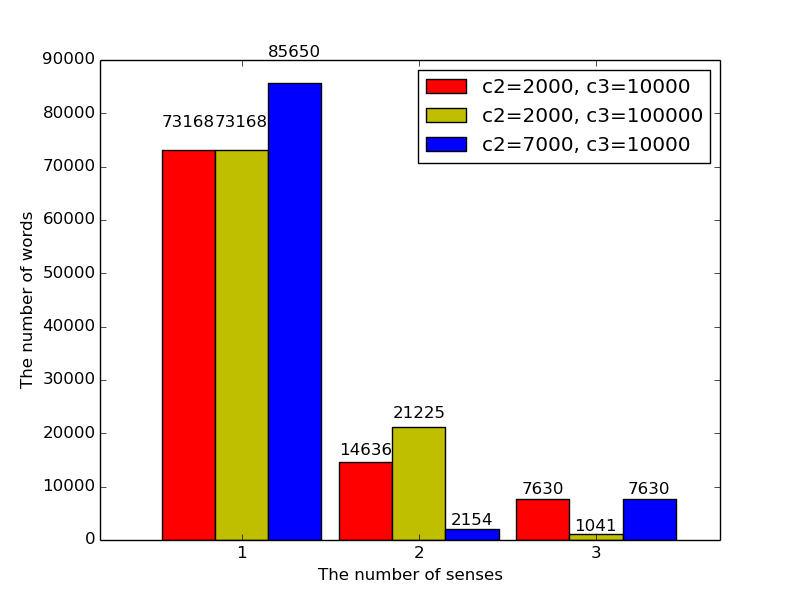
\includegraphics[width=0.8\textwidth]{sensecount} 
	\caption{sensecount}
	\label{fig:sensecount}
\end{figure}


\paragraph{Different Learning Rate and Gamma} \ \\
Table \ref{tab:group4} shows that ...

\begin{table}[tb]

\caption{Different Learning Rate and Gamma Comparison} \label{tab:group4} 
\begin{center}
\begin{tabular}{|l|l|l|l|l|l|l|l|l|l|l|}
\hline
id& lr & gm & $t1$ & $t2$ & iter & $t3$ & $t4$ &    loss  & 	SCWS & 	word353	  \\ 
\hline
7	& 0.1		& 0.9		& 849	& 343	& 35	& 1838 &	64335  & 0.246 &0.4371	&0.4891	  \\ 
\hline
8	& 0.01		& 0.95		& 797	& 370	& 40	& 1851 &	74032  & 0.267 &..	&..	  \\ 
\hline
\end{tabular}
\end{center}
\end{table}
\clearpage

\paragraph{Different Number of Output Senses Syn1}  \ \\
From Table~\ref{tab:group5}, it is very obvious that if syn1 has multiple sense embeddings (output embeddings), the final loss is much smaller, although it needs more time to achieve convergence. After inspection the closest neighbors of senses the reason got clear. Say there are two words, e.g. "bank" and "money" with multiple senses. Then if money$_1$ was a close neighbor of bank$_0$ then it turned out that money$_0$ was a close neighbor of bank$_1$. Hence the closest senses were simply permuted, and the senses were not really meaningful. Hence we concluded that there should be only one output sense for each word. This will avoid this effect. 



\begin{table}[tb]

\caption{Comparison of the different number of output senses Syn1} \label{tab:group5} 
\begin{center}
\begin{tabular}{|l|l|l|l|l|l|l|l|l|l|}
\hline
id& syn1 & $t1$ & $t2$ & iter & $t3$ & $t4$ &    loss  & 	SCWS & 	word353	   \\ 
\hline
7	& true		& 849	& 343	& 35	& 1838 &	64335 & 0.2457 &0.4371	&0.4891	   \\ 
\hline
11 	& false		& 1192	& 365	& 45	& 2866 &	128949 & 0.2069 & & 0.4802  \\ 
\hline
\end{tabular}
\end{center}
\end{table}
 

\begin{table}[tb]
\caption{Nearest words comparison} \label{tab:nearestcompare} 

\begin{center}
\begin{tabular}{ |l|l|l| }
\hline
 & id 7 , one sense output embedding& id 11, multiple senses output embedding \\
\hline
\hline
\multirow{3}{*}{apple} 
 & cheap, junk, scrap, advertised 				& kodak, marketed, nokia, kit \\
 & chocolate, chicken, cherry, berry 		& portable, mgm, toy, mc \\
 & macintosh, linux, ibm, amiga			& marketed, chip, portable, packaging \\ 
 \hline
\multirow{3}{*}{bank} 
 & corporation, banking, banking, hsbc & trade, trust, venture, joint \\
 & deposit, stake, creditors, concession & trust, corporation, trade, banking \\ 
 & banks, side, edge, thames &  banks, border, banks, country \\ 
 \hline
\multirow{3}{*}{cell} 
 & imaging, plasma, neural, sensing & dna, brain, stem, virus \\
 & lab, coffin, inadvertently, tardis & cells, dna, proteins, proteins \\
 & cells, nucleus, membrane, tumor & dna, cells, plasma, fluid \\
\hline
\end{tabular}
\end{center}
\end{table}

\subsection{Comparison to prior analyses}
Here you have to compare to the results similarity analysis results of \cite{MikolovSutskeverEtAl2013} and \cite{HuangSocherEtAl2012}.\com{todo!!!!}

\com{A possible final verdict: Due to the little time left no thorough experiments could be performed. Spark parameters have to be tuned to distribute the calculations over multiple computing machines. The number of iterations as well as the schedule for reducing the learning rate has to be explored. If there is more time then the results should get much better.}
 
\section{Case Analysis}

\begin{table}[tb]
	\caption{Sense Similarity Matrix of $apple$} \label{tab:sensematrixapple} 
	\begin{center} \begin{tabular}{|l|l|l|l|}  
			\hline
			& $apple_0$ & $apple_1$ & $apple_2$ \\ 
			\hline  
			$apple_0$  & 1.000000  & 0.788199 & 0.800783 \\ 
			\hline 
			$apple_1$  & 0.788199 & 1.000000 & 0.688523  \\ 
			\hline 
			$apple_2$  & 0.800783 & 0.688523 & 1.000000  \\
			\hline
		\end{tabular} 
	\end{center}
\end{table}
In the following, we will select only one experiment's result to do the visualization of senses and compute nearest word senses. The selection is based on the final loss and similarity task, specifically it is experiment 7 from above.   

\begin{table}[tb]
	
	\caption{Nearest Words of $apple$} \label{tab:nearestapple} 
	\begin{center} \begin{tabular}{|l|l|}  
			\hline 
			$apple_0$: & cheap , junk , scrap , advertised , gum , liquor , pizza   \\  
			\hline
			$apple_1$: & chocolate, chicken, cherry, berry, cream, pizza, strawberry  \\  
			\hline
			$apple_2$: & macintosh, linux, ibm, amiga, atari, commodore, server   \\  
			\hline
		\end{tabular}
	\end{center}
\end{table}

Firstly we give the result for the word $apple$, where different sense are quite nicely separated. Table \ref{tab:sensematrixapple} shows the sense similarity matrix of $apple$. The similarity value is the cosine similarity between two embedding vectors. Table \ref{tab:nearestapple} shows the nearest words of different senses from $apple$. We can see that $apple_0$ and $apple_1$ are about food. They are similar somehow. And $apple_2$ is about the computer company. The next are some sentence examples including the word $apple$ in Table \ref{tab:sentenceapple}. These are the sentences containing the assigned word senses from the last iteration of training. To make it clear, we only display the sense label of the $apple$, although the other words also have multiple senses.

To visualize semantic neighborhoods we selected 100 nearest words for each sense of $apple$ and use t-SNE algorithm \citep{MaatenHinton2008} to project the embedding vectors into two dimensions. And then we only displayed $70\%$ of words randomly to make visualization better, which is shown in Figure \ref{fig:apple}. And we use another table (Table ..) to show the comparison of with other two models (huang and em).
 


\begin{table}[tb]

\caption{Sentence Examples of $apple$} \label{tab:sentenceapple} 
\begin{center} 
\begin{tabular}{|l|l|}
\hline
\multirow{2}{*}{$apple_0$} 
&he can't tell an onion from an \textcolor{red}{$apple_0$} and he's your eye witness\\
&some fruits e.g \textcolor{red}{$apple_0$} pear quince will be ground\\
\hline
\multirow{2}{*}{$apple_1$} 
&the cultivar is not to be confused with the dutch rubens \textcolor{red}{$apple_1$}\\
&the rome beauty \textcolor{red}{$apple_1$} was developed by joel gillette \\
\hline
\multirow{2}{*}{$apple_2$} 
&a list of all \textcolor{red}{$apple_2$} internal and external drives in chronological order\\
&the game was made available for the \textcolor{red}{$apple_2$} iphone os mobile platform\\
\hline
\end{tabular} 
\end{center}
\end{table}


\begin{figure}[tb]
	\caption{Nearest words from $apple$}
  \centering
	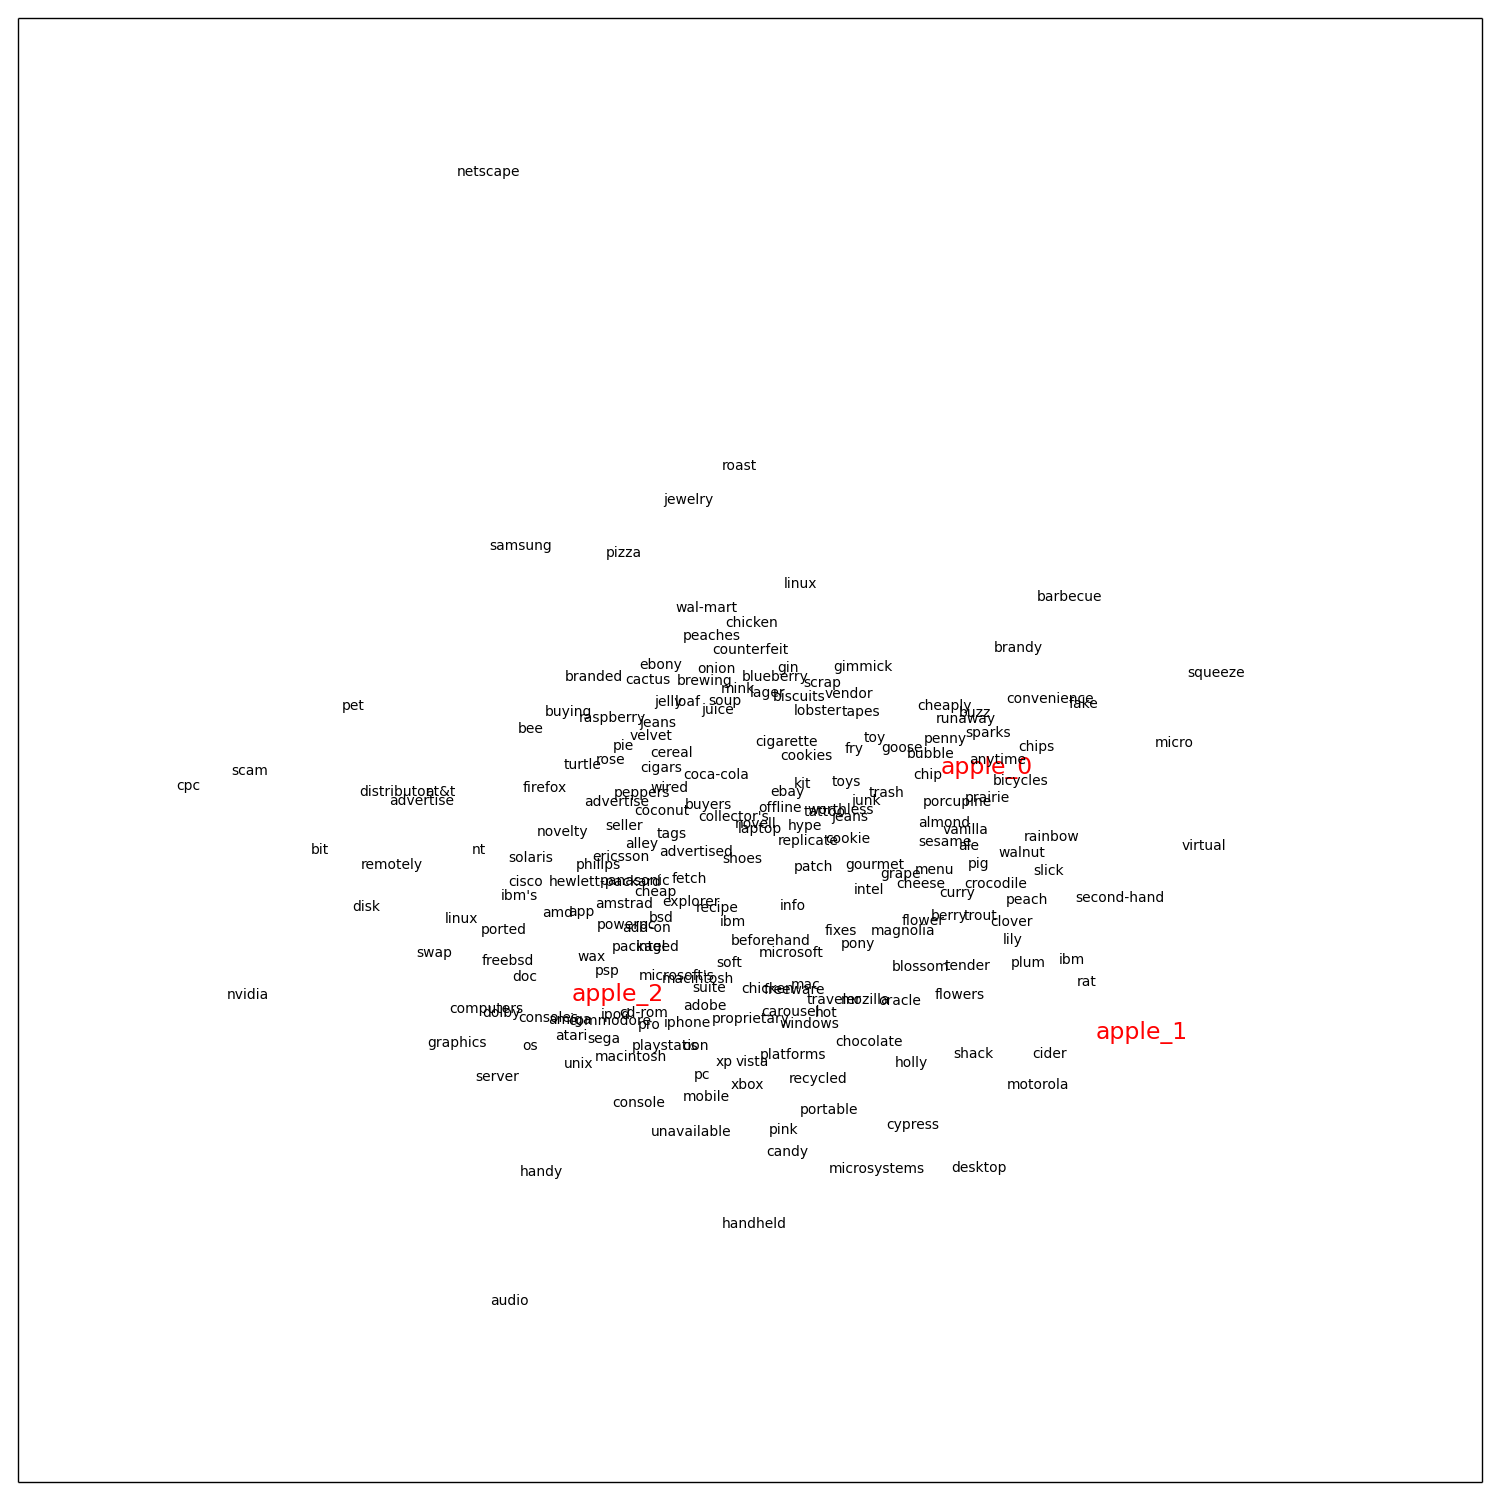
\includegraphics[width=1.0\textwidth]{apple} 
	\label{fig:apple}
\end{figure}

\clearpage % force floats to be dislayed

\paragraph{} Next, we select other 5 words $fox$ , \ $net$ , \ $rock$ , \ and $plant$, and list nearest words to each of their 3 senses in Table \ref{tab:nearestwordsother}. Each line contains the nearest words for one of the senses. This table nicely illustrates the different meanings of words: 
\begin{itemize}
	\item fox: Sense 1 and 2 cover different movies and film directors while sense 3 is close to tv networks.
	\item net: Sense 1 is related to communication networks, sense 2 to profits and earnings and sense 3 to actions
	\item rock: Sense 1 and sense 2 is related to music while sense 3 to stone.
	\item run: Sense 1 is related to election campains, sense 2 expresses the movement and sense 3 to public transport.
	\item plant: Sense 1 is close to biologic plants and small animals, sense 2 is related to flowers and sense 3 to factories.
\end{itemize}


In table \ref{tab:sentenceother} we show one example sentence for each sense.
The example sentences are also cut by ourself without affecting the meaning of the sentence. It's not difficult to find that $fox$ has meanings: ; $net$ has meanings: ; $rock$ has meanings: ; $plant$ has meanings: . 


\begin{table}[tb]
\caption{Nearest words from $fox$ , \ $net$ , \ $rock$ , \ $run$ and \ $plant$} \label{tab:nearestwordsother} 
\begin{center} 
\begin{tabular}{|l|l|}
\hline
\multirow{3}{*}{$fox$}   
& archie, potter, wolfe, hitchcock, conan, burnett, savage  \\ 
& buck, housewives, colbert, eastenders, howard, kane, freeze
 \\ 
& abc, sky, syndicated, cw, network's, ctv, pbs \\ 
\hline
\multirow{3}{*}{$net$}  
& generates, atm, footprint, target, kbit/s, throughput, metering   \\  
& trillion, rs, earnings, turnover, gross, euros, profit  \\  
&jumped, rolled, rebound, ladder, deficit, snapped, whistle   \\  
\hline 
\multirow{3}{*}{$rock$}  
&echo, surf, memphis, strawberry, clearwater, cliff, sunset  \\  
& r$\,$b, hip, roll, indie, ska, indie, hop  
 \\  
&formations, crust, melting, lava, boulders, granite, dust   \\  
\hline 
\multirow{3}{*}{$run$}
& blair, taft, fraser, monroe, precinct, mayor's, governor's  \\  
& streak, rushing, tying, shutout, inning, wicket, kickoff
 \\  
& running, tram, travel, express, trams, inbound, long-distance \\
\hline  
\multirow{3}{*}{$plant$}
& plants, insect, seeds, seed, pollen, aquatic, organic  \\  
& flowering, orchid, genus, bird, species, plants, butterfly
 \\  
& electricity, steel, refinery, refinery, manufacturing, gas, turbine  \\
\hline
\end{tabular}
\end{center}
\end{table}


\begin{table}[tb]
\caption{Sentence Examples of $fox$ , \ $net$ , \ $rock$ , \ $run$ and \ $plant$ } \label{tab:sentenceother} 
\begin{center} 
\begin{tabular}{|l|l|}
\hline
\multirow{3}{*}{$fox$} 
&run by nathaniel mellors dan \textcolor{red}{$fox_0$} andy cooke and ashley marlowe\\
&he can box like a \textcolor{red}{$fox_1$} he's as dumb as an ox\\
&the grand final was replayed on fox sports australia and the \textcolor{red}{$fox_2$} footy channel\\
\hline
\multirow{3}{*}{$net$} 
&\textcolor{red}{$net_0$} supports several disk image formats partitioning schemes\\
&in mr cook was on the forbes with a \textcolor{red}{$net_1$} worth of billion \\
&nothin but \textcolor{red}{$net_2$} freefall feet into a net below story tower\\
\hline
\multirow{3}{*}{$rock$} 
&zero nine is a finnish hard \textcolor{red}{$rock_0$} band formed in kuusamo in\\
&matt ellis b december is a folk \textcolor{red}{$rock_1$} genre singer-songwriter\\
&cabo de natural park is characterised by volcanic \textcolor{red}{$rock_2$} formations\\
\hline
\multirow{3}{*}{$run$} 
&dean announced that she intends to \textcolor{red}{$run_0$} for mayor again in the november election\\
& we just couldn't \textcolor{red}{$run_1$} the ball coach tyrone willingham said\\
& the terminal is \textcolor{red}{$run_2$} by british rail freight company ews\\
\hline
\multirow{3}{*}{$plant$} 
&these phosphoinositides are also found in \textcolor{red}{$plant_0$} cells with the exception of pip\\
&is a genus of flowering \textcolor{red}{$plant_1$} in the malvaceae sensu lato\\
&was replaced with a new square-foot light fixture \textcolor{red}{$plant_2$} in sparta tn\\
\hline
\end{tabular} 
\end{center}
\end{table}


\paragraph{} Finally, for each sense of each word ($apple$, $fox$,$net$,$rock$ and $plant$), we select only the 20 nearest words, and combine them together to do another t-SNE embeddingof  two dimensions. The the result is shown in Figure \ref{fig:keywords20}. 

\begin{figure}[tb]
  \centering
	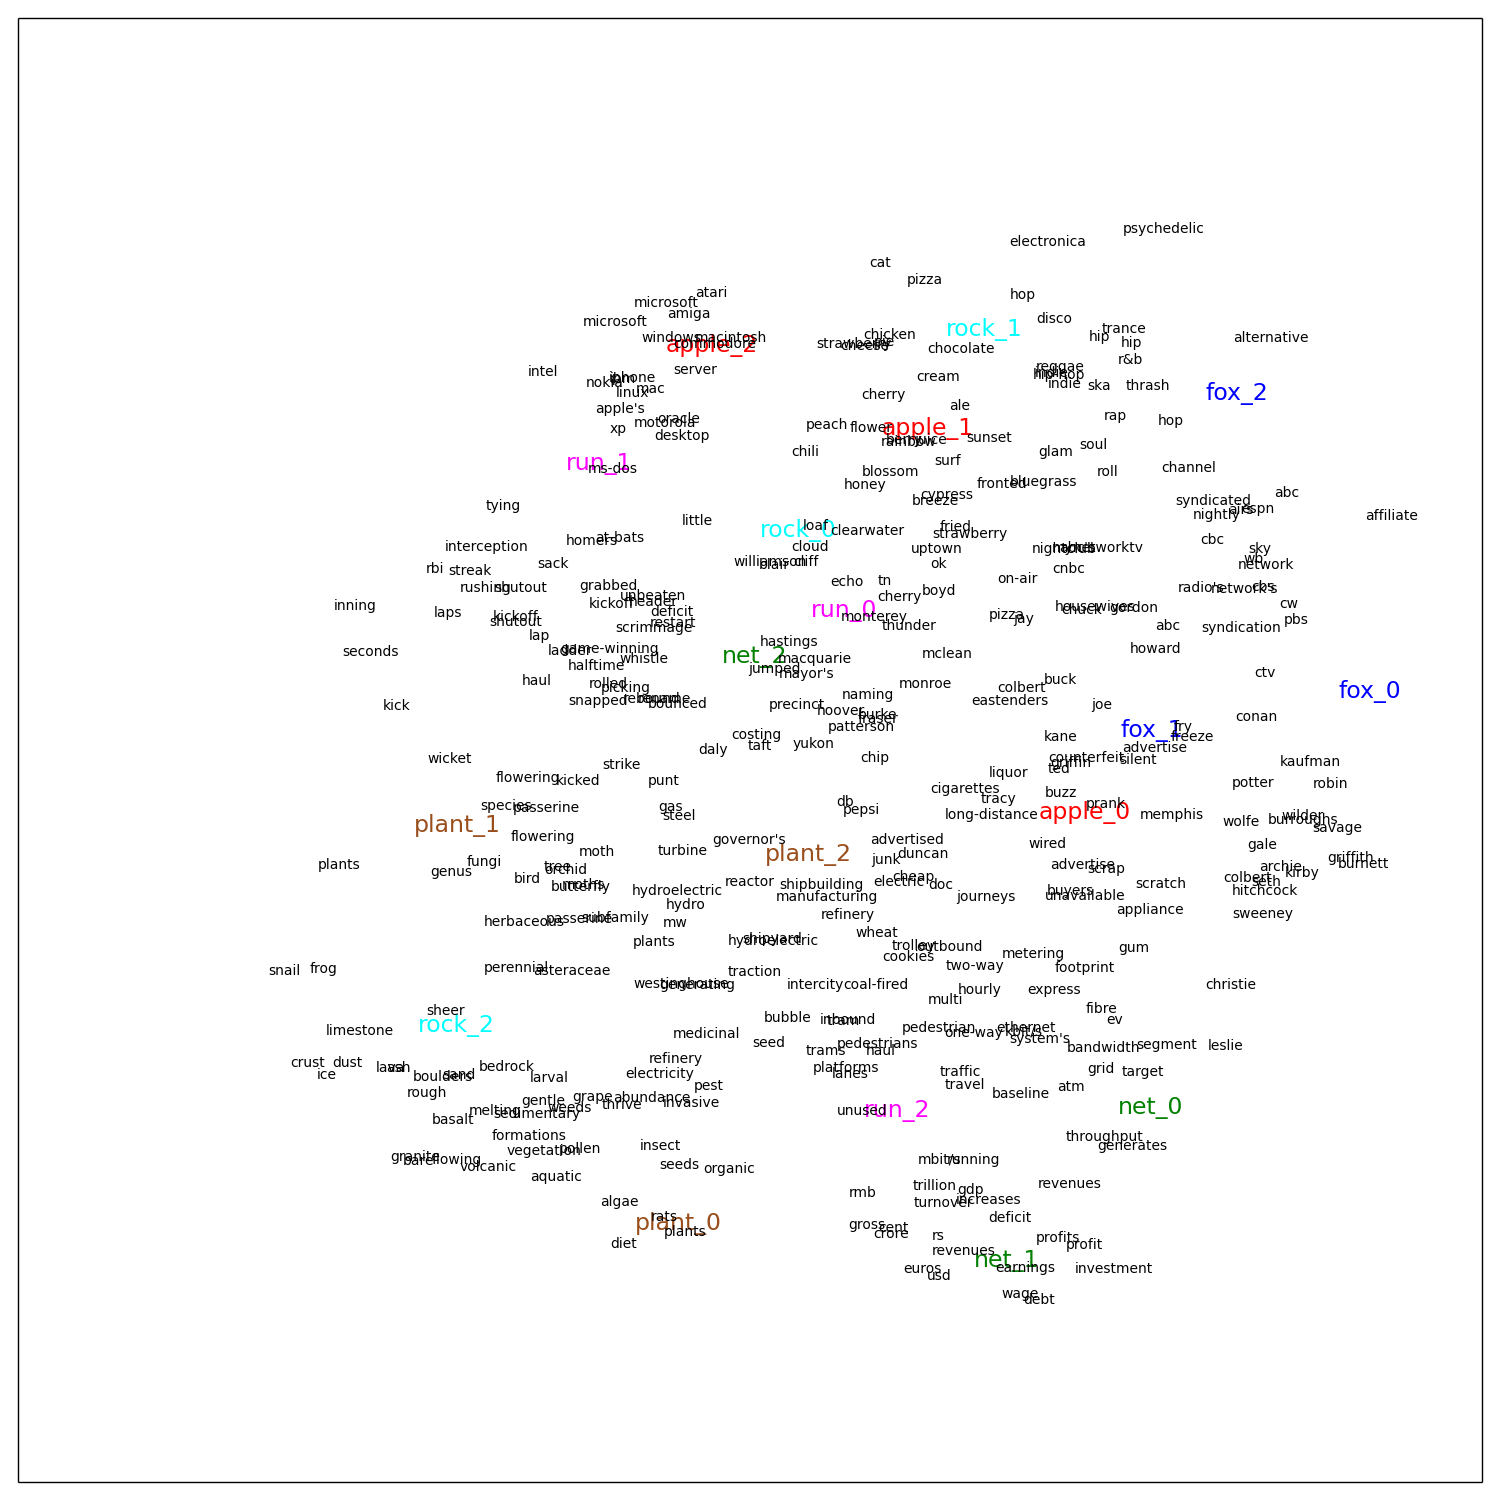
\includegraphics[width=1.0\textwidth]{some20} 
	\caption{Nearest words from $apple$,\ ,$fox$,\ ,$net$,\ ,$rock$,\  , $run$ and $plant$}
	\label{fig:keywords20}
\end{figure}

\paragraph{} From these visualization, we can say our model is able to extract meaningful sense vectors which may be used for subsequent analyses. There is, however, room for improvement.
